\documentclass[table]{beamer}
\usetheme{gpmeet}
\graphicspath{{../../figures/}}

\newcommand{\leftRect}[2]{\node[draw=text,very thick,rounded corners, text width=0.46\textwidth,minimum height=6cm] at (0,0) {\centering\textbf{#1}\\ \raggedright \color{text}#2};}
\newcommand{\rightRect}[2]{\node[draw=text,very thick,rounded corners, text width=0.46\textwidth,minimum height=6cm] at (0.54\textwidth,0) {\centering\textbf{#1}\\ \raggedright \color{text}#2};}

\usepackage{tikz}

\title{Group meetings}

\subtitle{Memristors-based recurent modules for neural computing}

\author[V. BARBAZA]{Valentin BARBAZA}

\date{23/09/2023}

\logo{
  \begin{tikzpicture}[overlay,remember picture]
    \node[left=0cm] at (current page.34){
      
\includegraphics[height=1cm]{logos/ist.eps}
      \hspace{1pt}
      
\includegraphics[height=1cm]{logos/inesc-mn.png}
      
\includegraphics[height=1cm]{logos/inesc-id.eps}
    };
  \end{tikzpicture}
}

\begin{document}

\frame{\titlepage}


\begin{frame}
  \frametitle{Introduction}

  \begin{itemize}
      \color{text}
    \item I am working on an analog implementation of a LSTM Neural Networks.
    \item The final objective of my thesis is to have a successful simulation of such a circuit.
  \end{itemize}

\end{frame}

\begin{frame}
  \frametitle{Introduction}
  \centering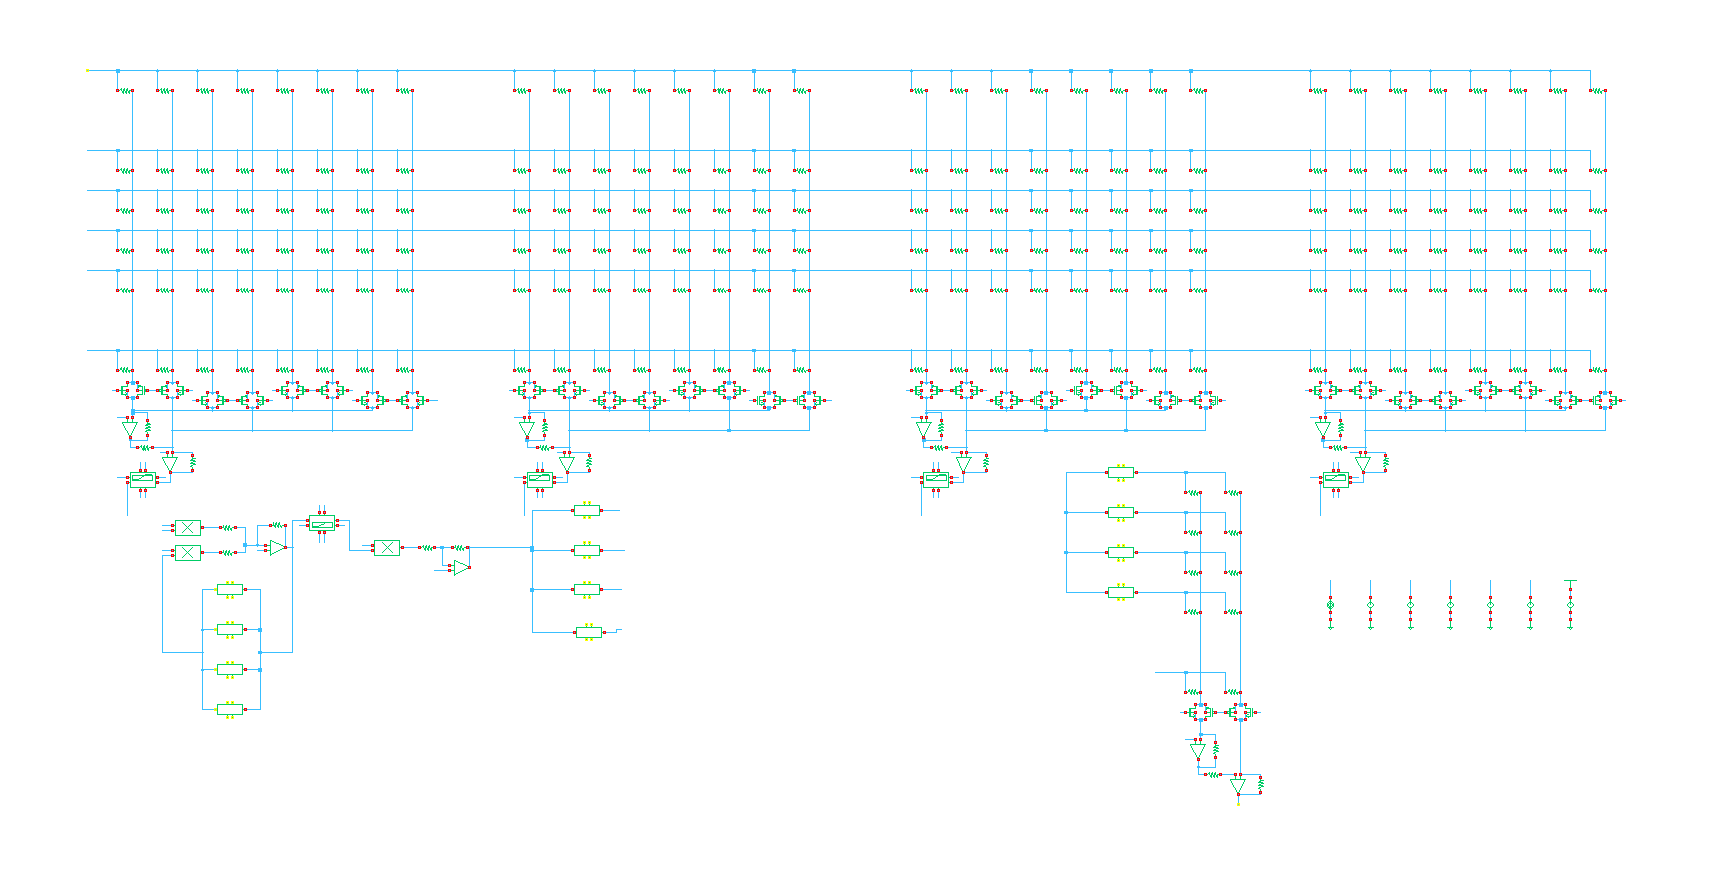
\includegraphics[width=\textwidth]{lstm/lstm-np}
\end{frame}

\begin{frame}
  \frametitle{Last weeks...}

  There was no meeting last week, and a lot happened but here is what I'm doing :
  \begin{itemize}
    \item Mainly focused on writing the thesis
    \item I also need to run a new simulation with a new problem
  \end{itemize}
\end{frame}

\begin{frame}{What's new}
  \begin{itemize}
    \item Results obtianed :
      \begin{itemize}
          \color{text}
        \item None yet
      \end{itemize}
    \item Improvements :
      \begin{itemize}
          \color{text}
        \item
      \end{itemize}
    \item Relevant information :
      \begin{itemize}
          \color{text}
        \item
      \end{itemize}
  \end{itemize}
\end{frame}

\begin{frame}
  \frametitle{Problems/doubts}
  \begin{itemize}
    \item What is the approximate onChip area of an opAmp
    \item What is the precision of a memristor when setting the resistance
    \item I feel like my state of the art is missing content...
    \item When would my thesis defense happen ?
    \item I'm afriad i might not have time to finish on time wiht enough content.
  \end{itemize}
\end{frame}

\begin{frame}{Next weeks}

  List of what I plan to do in the next weeks :

  \centering
  \rowcolors{2}{evenRow}{oddRow}
  \begin{tabular}{ c m{6cm} }
    \rowcolor{firstRow}
    \color{white}\textbf{\#} & \centering\color{white}Task \cr
    0 & Work on thesis \\
    1 & Figure out the new problem \\
    2 & Digital inference time \\
  \end{tabular}
\end{frame}

\begin{frame}{Networking and sharing}
  \begin{tikzpicture}
    \leftRect{Help/Collaboration :}{- I'm looking for a software to create nice looking electronic circuit.}

    \rightRect{Recommendations :}{None}
  \end{tikzpicture}
\end{frame}

\end{document}
